Having explored existing data models and tested their limitations against several case studies from the Middle Ages, we propose a model with the entities and relationships represented in Figure \ref{fig:ProposedEntities}. To begin, we present all the entities we believe necessary for a data model tasked with organizing and delivering information about texts and traditions in Medieval literature, particularly texts about chivalric tales and legends. Then, we list all the attributes each entity features. Compared to the former, this latter section is more likely to need renegotiation based on the idiosyncratic qualities of different literary corpora.

\subsection{Entity relationships}

In Section \ref{sec:basicER}, we start by simply introducing the entities' names and the nature of their relationships to one another. Subsequently, we present a technical schematic of the entities' relationships to one another.

\subsubsection{Nature of the relationships between entities}
\label{sec:basicER}

In Figure \ref{fig:ProposedEntities}, we see that one \textit{Cycle} can be a part of another \textit{Cycle} via the foreign-key relationship ``is part of.'' This is case when one the subject of one \textit{Cycle}, such as \textit{Works} about Charlemagne's knight Agolant, can also be interpretted as being a part of a larger \textit{Cycle}, such as a \textit{Cycle} about Charlemagne broadly. Thus, due to \textit{Cycles'} potential inter-entity connections, the same relationship ``is part of'' applies to \textit{Cycles} and to \textit{Works}. In our proposed model, a \textit{Cycle} can have only one parent \textit{Cycle} and a \textit{Work} belongs to the tradition of only one \textit{Cycle}. Both of these relationships are optional.

\begin{figure}[ht]
    \begin{center}
        \tikzstyle{s} = [rectangle, rounded corners, minimum width=2cm, text width=2cm, minimum height=1cm, text centered, draw=black]
\tikzstyle{arrow} = [thick,->,>=stealth]
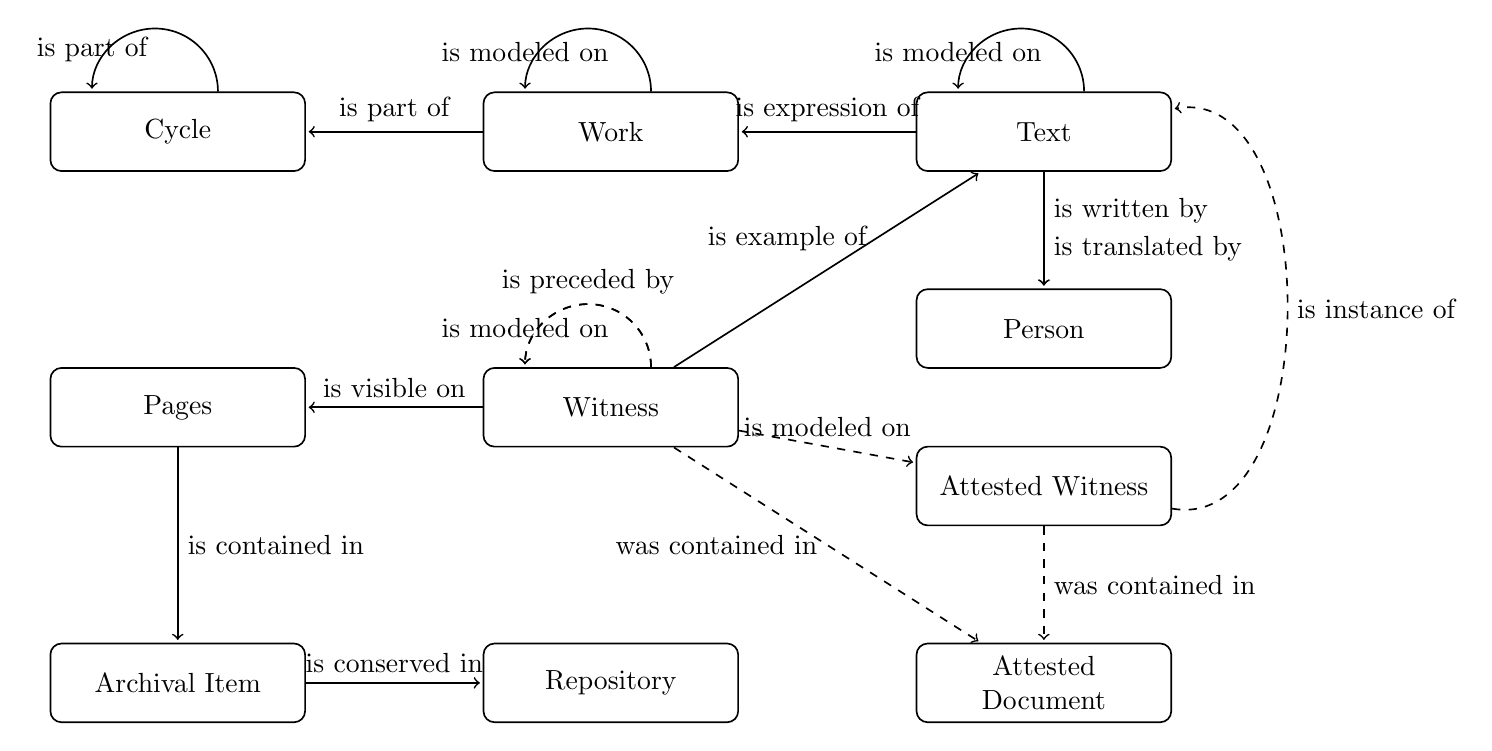
\begin{tikzpicture}[-,shorten >=1pt,auto,node distance=2.5cm,semithick]
\tikzstyle{every state}=[fill=red,draw=none,text=white]

\node[s] (cycle) [] {Cycle};
\node[s] (work) [right of=cycle, xshift=3cm] {Work};
\node[s] (text) [right of=work, xshift=3cm] {Text};

\node[s] (person) [below of=text] {Person};

\node[s] (attestedWitness) [below of=person, yshift=0.5cm] {Attested Witness};

\node[s] (witness) [below of=work, yshift=-1cm] {Witness};

\node[s] (pages) [left of=witness, xshift=-3cm] {Pages};

\node[s] (item) [below of=pages, yshift=-1cm] {Archival Item};

\node[s] (repo) [right of=item, xshift=3cm] {Repository};

\node[s] (document) [right of=repo, xshift=3cm] {Attested Document};

% \draw[dashed, ->] (witness.-45) arc (200:475:8mm) 
%   node[pos=0.5, below] () {is preceded by};
\draw[dashed, ->] (witness.45) arc (0:180:8mm)
  node[above, pos=0.5] () {is preceded by};
\draw[dashed, ->] (witness.45) arc (0:180:8mm)
  node[above, yshift=0.25cm] () {is modeled on};
\draw[->] (cycle.45) arc (0:180:8mm) 
  node[above, yshift=0.25cm] () {is part of};
\draw[->] (work.45) arc (0:180:8mm) 
  node[above, yshift=0.25cm] () {is modeled on};
\draw[->] (work) -- (cycle)
  node[pos=0.5, above] () {is part of};
\draw[->] (text) -- (work)
  node[pos=0.5, above] () {is expression of};
\draw[->] (witness) -- (text)
  node[pos=0.66, left] () {is example of};
\draw[dashed,->] (witness) -- (document)
  node[pos=0.5, left] () {was contained in};
\draw[->] (pages) -- (item)
  node[pos=0.5, right] () {is contained in};
\draw[->] (witness) -- (pages)
  node[pos=0.5, above] () {is visible on};
\draw[->] (item) -- (repo)
  node[pos=0.5, above] () {is conserved in};
\draw[->] (text.45) arc (0:180:8mm) 
  node[yshift=0.25cm, above] () {is modeled on};
\draw[->] (text) -- (person)
  node[pos=0.66, right] {is translated by};
\draw[->] (text) -- (person)
  node[pos=0.33, right] {is written by};
\draw[dashed, ->] (witness) -- (attestedWitness)
  node[pos=0.5, above] {is modeled on};
\draw[dashed, ->] (attestedWitness) -- (document)
  node[pos=0.5, right] {was contained in};

\path[every node]
  (attestedWitness) edge[dashed, ->, bend right=100] node [pos=0.5, right] {is instance of} (text)
  ;

\end{tikzpicture}
    \end{center}
\caption{Proposed Entities}
\label{fig:ProposedEntities}
\end{figure}

The \textit{Text} entity can have five relationships, three of which originate from it, as seen in Figure \ref{fig:ProposedEntities}. First, a \textit{Text} must relate to one and only one \textit{Work}. According to our definition, the \textit{Text} is the expression in a certain human language and literary style of a \textit{Work}. One \textit{Text} can be modeled on or the translation of an anterior \textit{Text}. Furthermore, a \textit{Text} can optionally be related to one or more \textit{Person} entities. The latter can be responsible either for authoring the \textit{Text} or for translating it. Finally, a \textit{Text} should have at least one \textit{Witness} or \textit{Attested Witness} relate to it; otherwise, we would have no evidence of the abstract \textit{Text} entity's existence. However, the relationship between a \textit{Text} and either of the two types of witnesses (extant \textit{Witness} and lost \textit{Attested Witness}) stems from the latter and is not a requirement for the \textit{Text} entity.

Originating from the extant \textit{Witness} are potentially five types of entity relationships. First and foremost, a \textit{Witness} must relate to one and only one \textit{Text}. By definition, a \textit{Witness} is a version of the text's linguistic content, spelled out in a sequence of characters, as demonstrated in Table \ref{tab:TextVersions}. Second, the \textit{Witness}, by virtue of being extant and not a lost \textit{Attested Witness}, must be visible on the \textit{Pages} of an \textit{Archival Item}. When it has survived through fragments, one \textit{Witness} can relate to another through the attribute ``is preceded by.'' This is the case when one fragment is presumed to have come after another fragment, as demonstrated in the Table \ref{tab:CampsAspremont}.

Finally, and again optionally, a \textit{Witness} can have formerly been contained in a document which has not survived but to whose historical existence scholars attest based on philological and codicological evidence. The latter document is the entity \textit{Attested Document} and it receives a relationship from one or more \textit{Witnesses} that it is alleged to have transmitted together. The \textit{Attested Document} can also have contained a lost \textit{Attested Witness}. As sometimes mentioned in archival catalogues, an extant \textit{Witness} might have been modeled on a presumed version of a \textit{Text} that has since been lost, an \textit{Attested Witness}. As such, a \textit{Witness} can have a relationship to an \textit{Attested Witness}.

\textit{Pages} represents an uninterrupted set of pages and, when digitized, images of an \textit{Archival Item} on which the text content of a \textit{Witness} can be read. In our data model, a \textit{Pages} entity, which depends on an extant \textit{Witness}, must be contained in an \textit{Archival Item}. The \textit{Archival Item} can relate to multiple \textit{Pages} entities. However, the first folio of one \textit{Pages} entity must not come before the last folio of another \textit{Pages} entity in the same \textit{Archival Item}. In other words, \textit{Pages} entities cannot overlap. They represent a unique set of leafs or pages in an \textit{Archival Item}, and they present the content of only one \textit{Witness}. Lastly, the \textit{Archival Item}, being an object one can consult and which continues to persist, contrary to the \textit{Attested Document}, must be conserved in a \textit{Repository}.

% \subsection{Entity-relationship diagram}
% \label{sec:ERDiagram}

% \begin{figure}[ht]
%     \begin{center}
%         \tikzstyle{s} = [rectangle, rounded corners, minimum width=2cm, text width=3cm, minimum height=1cm, text centered, draw=black]
\tikzstyle{arrow} = [thick,->,>=stealth]
\begin{tikzpicture}[-,shorten >=1pt,auto,node distance=1.5cm,semithick]
\tikzstyle{every state}=[fill=red,draw=none,text=white]

\pic [] { entityassociative = {{cycle}
{\textbf{Cycle}}
{
  \textbf{Cycle} (is part of) \\
}
}};

\pic [right = 10em of cycle] { entityassociative = {{work}
{\textbf{Work}}
{
  \textbf{Cycle} FK \\
}
}};

\pic [right = 10em of work] { entityassociative = {{text}
{\textbf{Text}}
{
  \textbf{Work} FK \\
  \textbf{Person} FK \\
  \textbf{Text} (is modeled on, is translation of) \\
}
}};

\pic [below = 6em of work] { entityassociative = {{witness}
{\textbf{Witness}}
{
  \textbf{Text} FK \\
  \textbf{Attested Document} FK \\
  \textbf{Witness} (is preceded by) \\
}
}};

\pic [left = 10em of witness] { entityassociative = {{pages}
{\textbf{Pages}}
{
    \textbf{Witness} FK \\
    \textbf{Archival Item} FK \\
}
}};

\pic [below = 8em of text] { entityassociative = {{person}
{\textbf{Person}}
{
}
}};

\pic [below = 5em of pages] { entityassociative = {{item}
{\textbf{Archival Item}}
{
    \textbf{Repository} FK \\
}
}};

\pic [right = 10em of item] { entityassociative = {{repo}
{\textbf{Repository}}
{
}
}};

\pic [right = 10em of repo] { entityassociative = {{document}
{\textbf{Attested Document}}
{
}
}};

\draw[one-omany] (cycle) -- node[above, pos=0.66]{is part of} (work);
\draw[one-omany] (text) -- node[right, yshift=-0.1cm, pos=0.8]{is instance of} (witness);
\draw[one-omany] (witness) -- node[above, pos=0.66]{contains} (pages);
\draw[one-many] (work) -- node[above, pos=0.66]{is instance of} (text);
\draw[omany-omany] (text) -- node[right, pos=0.25]{is translated by} (person);
\draw[omany-omany] (text) -- node[right, pos=0.5]{is written by} (person);
\draw[many-one] (pages) -- node[right, pos=0.25]{is contained in} (item);
\draw[omany-one] (item) --node[above, pos=0.40]{is conserved in} (repo);
\draw[omany-one] (witness) -- node[right, yshift=0.1cm, pos=0.15]{was contained in} (document);

\end{tikzpicture}
%     \end{center}
% \label{fig:AllER}
% \caption{Entities, their foreign key (FK) relationships, and cardinality.}
% \end{figure}

%%%%%%%%%%%%%%%%%%%%%%%%%

\subsection{Cycle}

Definition: General theme that a group of \textit{Works} can share.  

\vspace{1em}
\noindent Attributes:
\begin{itemize}
    \item \texttt{title} (text, req., uniq.): Received name of the \textit{Cycle}, either in the language of the first known \textit{Text} to treat the matter or in the language most used in scholarship.
    \item \texttt{is part of} (foreign key, \textbf{Cycle}, opt., uniq.): The meta-\textit{Cycle}, of which the \textit{Cycle} is a part.
\end{itemize}

\begin{figure}[ht]
    \begin{center}
        \tikzstyle{s} = [rectangle, rounded corners, minimum width=2cm, text width=3cm, minimum height=1cm, text centered, draw=black]
\tikzstyle{arrow} = [thick,->,>=stealth]
\begin{tikzpicture}[-,shorten >=1pt,auto,node distance=1.5cm,semithick]
\tikzstyle{every state}=[fill=red,draw=none,text=white]

\pic [] { entityassociative = {{cycle}
{\textbf{Cycle}}
{
  \textbf{ID} \\
  \hline
  title \\
  is part of \\
}
}};

\pic [right = 15em of cycle] { entityassociative = {{work}
{\textbf{Work}}
{
  \textbf{ID} \\
  \hline
  title \\
  is part of \\
}
}};


\draw[one-many] (cycle.east) -- node[label, above]{Cycle has 1 or more} (work.west);
\draw[one-many] (cycle.east) -- node[label, below]{Works that are part of it}(work.west);

\end{tikzpicture}
    \end{center}
\label{fig:CycleER}
\caption{\textit{Cycle} entity relationships.}
\end{figure}

%%%%%%%%%%%%%%%%%%%%%%%%%

\subsection{Work}

Definition: Content of a story, which has a recognizable structure and can be recounted in different ways while remaining the same story.

\vspace{1em}
\noindent Attributes:
\begin{itemize}
    \item \texttt{title} (text, req., uniq.): Received name of the \textit{Work}, either in the language of the first known \textit{Text} to treat the matter or in the language most used in scholarship.
    \item \texttt{is part of} (foreign key, \textbf{Cycle}, opt., uniq.): The \textit{Cycle}, of which the \textit{Work} is a part.
    \item \texttt{is modeled on} (foreign key, \textbf{Work}, opt., uniq.): If a reworking of an anterior \textit{Work}, the \textit{Work} on which it is modeled.
\end{itemize}


\begin{figure}[ht]
    \begin{center}
        \tikzstyle{s} = [rectangle, rounded corners, minimum width=2cm, text width=3cm, minimum height=1cm, text centered, draw=black]
\tikzstyle{arrow} = [thick,->,>=stealth]
\begin{tikzpicture}[-,shorten >=1pt,auto,node distance=1.5cm,semithick]
\tikzstyle{every state}=[fill=red,draw=none,text=white]

\pic [] { entityassociative = {{cycle}
{\textbf{Cycle}}
{
  \textbf{ID} \\
  \hline
  title \\
  is part of \\
}
}};

\pic [right = 12em of cycle] { entityassociative = {{work}
{\textbf{Work}}
{
  \textbf{ID} \\
  \hline
  title \\
  is part of \\
  is modeled on \\
}
}};


\pic [right = 12em of work] { entityassociative = {{text}
{\textbf{Text}}
{
  \textbf{ID} \\
  \hline
  is expression of \\
  is modeled on \\
  title \\
  person creator \\
  person translator \\
  creation date \\
  creation date text \\
  creation date cite \\
  matter \\
  regional genre\\
  language\\
  form\\
  poetic meter\\
  rhyme type \\
  strophe count \\
  strophe length \\
  verse length \\
}
}};

\pic [below = 5em of work] { entityassociative = {{reference}
{\textbf{Reference}}
{
  entity type\\
  entity ID \\
  unique identifier \\
  identifier source \\
  citation \\
}
}};

\draw[omany-omany] (reference) -- node[label, left, pos=0.5]{Work has 0, 1, or many References} (work);

\draw[one-omany] (cycle.east) -- node[label, above]{Work is part of} (work.west);
\draw[one-omany] (cycle.east) -- node[label, below]{1 and only 1 Cycle} (work.west);

\draw[one-many] (work.east) -- node[label, above]{Work has 1 or more} (text.west);
\draw[one-many] (work.east) -- node[label, below]{Text expressions} (text.west);

\end{tikzpicture}
    \end{center}
\label{fig:WorkER}
\caption{\textit{Work} entity relationships.}
\end{figure}

%%%%%%%%%%%%%%%%%%%%%%%%%

\subsection{Text}

Definition: Formulation of a \textit{Work} in human language, whose literary form and style can be detected and whose creation can be attributed to one or more individuals.

\vspace{1em}
\noindent Attributes:
\begin{itemize}
    \item \texttt{is expression of} (foreign key [\textbf{Work}], req., uniq.): The \textit{Work} that the \textit{Text} articulates.
    \item \texttt{is modeled on} (foreign key, [\textbf{Text}], opt., uniq.): If the \textit{Text} is derived from another \textit{Text}, a reference to the model \textit{Text}.
    \item \texttt{title} (text, req., uniq.): Either the given title of the \textit{Text}, as provided by the creator, or the standardized title most used in scholarship to refer to the \textit{Text}.
    \item \texttt{person creator} (foreign key [\textbf{Person}], opt., repeat.): The individual accredited with composing the \textit{Text}.
    \item \texttt{person translator} (foreign key [\textbf{Person}], opt., repeat.): When the \textit{Text} is a translation of another \textit{Text}, the individual accredited with creating the translation.
    \item \texttt{creation date} (list[date], opt., uniq.): A list of two or one dates; the first date is either the earliest or the only date associated with the \textit{Text's} creation, and the second date is the latest date associated with the creation.
    \item \texttt{creation date text} (text, opt., uniq.): The date associated with the \textit{Text's} creation as it is written in a scholarly source.
    \item \texttt{creation date cite} (text, opt., uniq.): A citation of the source that provided the date of creation.
    \item \texttt{matter} (terms, opt., repeat.): The matter treated in the \textit{Text}, as defined by Jean Bodel.
    \begin{itemize}
        \item \texttt{Breton}: Matter of Breton, which includes stories about Tristan and King Arthur.
        \item \texttt{France}: Matter of France, which includes stories about Charlemagne.
        \item \texttt{Rome}: Matter of Rome, which includes stories about Troy, Rome, Alexander, and antiquity.
    \end{itemize}
    \item \texttt{regional genre} (terms, req., uniq.): Literary genre attributed to the \textit{Text}.
    \begin{multicols}{2}
        \begin{itemize}
            \item Relevant to French tradition
                \begin{itemize}
                    \item \texttt{chanson de geste}\footcite[][]{Comfort1904}
                    \item \texttt{roman}\footcite[][]{Comfort1904}
                \end{itemize}
            \item Relevant to Middle Dutch tradition
                \begin{itemize}
                    \item \texttt{ridderepiek}\footcite[][]{kienhorst1988handschriften}
                    \item \texttt{ridderroman}
                \end{itemize}
            \item Relevant to Islandic tradition
                \begin{itemize}
                    \item \texttt{fornaldarsögur}
                    \item \texttt{riddarasögur}
                    \item \texttt{rímur}
                    \item \texttt{fornaldarrímur}
                    \item \texttt{riddararímur}
                \end{itemize}
            \item Relevant to Iberian tradition
            \item Relevant to Middle Irish tradition
            \item Relevant to Middle English tradition
            \item Relevant to Middle Welsh tradition
            \item Relevant to Middle High German tradition
            \item Relevant to Italian tradition
            \begin{itemize}
                \item \href{https://www.oxfordbibliographies.com/display/document/obo-9780195396584/obo-9780195396584-0199.xml}{\texttt{cantare}}
                \item \texttt{poema cavalleresche}
            \end{itemize}
        \end{itemize}
    \end{multicols}
    \item \texttt{language} (terms, req., uniq.): ISO code of the primary language through which the \textit{Text} expresses the \textit{Work}.
    \begin{multicols}{2}
        \begin{itemize}
            \item \texttt{ang}: Old English (ca. 450-1100)
            \item \texttt{cat}: Catalan
            \item \texttt{dum}: Middle Dutch
            \item \texttt{enm}: Middle English (1100-1500)
            \item \texttt{frk}: Frankish
            \item \texttt{frm}: Middle French (ca. 1400-1600)
            \item \texttt{fro}: Old French (842-ca. 1400)
            \item \texttt{fro\_ENG}: Old French in English dialect
            \item \texttt{fro\_ITA}: Old French in Italian dialect
            \item \texttt{fro\_PRO}: Medieval French in Provençal dialect
            \item \texttt{ghg}: Hiberno-Scottish Gaelic, Early Modern Irish
            \item \texttt{glg}: Galician
            \item \texttt{glg\_POR}: Galician in Portugese dialect
            \item \texttt{gmh}: Middle High German (ca. 1050-1500)
            \item \texttt{gml}: Middle Low German
            \item \texttt{goh}: Old High German (750-1050)
            \item \texttt{isl}: Islandic
            \item \texttt{ita}: Italian
            \item \texttt{mga}: Middle Irish (900-1200)
            \item \texttt{non}: Old Norse
            \item \texttt{non\_DAN}: East Norse, Old Danish
            \item \texttt{non\_SWE}: West Norse, Old Swedish
            \item \texttt{oco}: Old Cornish
            \item \texttt{odt}: Old Dutch
            \item \texttt{owl}: Old Welsh
            \item \texttt{por}: Portugese
            \item \texttt{pro}: Old Occitan, Old Provençal (to 1500)
            \item \texttt{spa}: Spanish or Castilian
            \item \texttt{sga}: Old Irish (to 900)
            \item \texttt{wlm}: Middle Welsh
            \item \texttt{xno}: Anglo-Norman
        \end{itemize}
    \end{multicols}
    \item \texttt{form} (terms, req., uniq.): Whether the \textit{Text} is formed in prose, verse, or a mix of both.
    \begin{multicols}{4}
        \begin{itemize}
            \item \texttt{prose}
            \item \texttt{verse}
            \item \texttt{mixed}
        \end{itemize}
    \end{multicols}
    \item \texttt{poetic meter} (terms, opt., uniq.): If the \textit{Text} is in verse, the type of poetic meter.
    \begin{multicols}{4}
        \begin{itemize}
            \item \texttt{alexandrines}
            \item \texttt{decasyllables}
            \item \texttt{hexasyllables}
            \item \texttt{octosyllables}
        \end{itemize}
    \end{multicols}
    \item \texttt{stanza length} (integer, opt., uniq.): If the \textit{Text} is in verse, the typical length of a stanza.\footnote{For example, in the Islandic tradition, \textit{Texts} that are of the \textit{ferskeytla} form are in four-line stanzas, \textit{braghenda} is in three lines, and the \textit{afhending} form is defined by the fact that they have two-line stanzas.}
    \item \texttt{verse length} (integer, opt., uniq.): If the \textit{Text} is in verse, the number of verses a complete version (\textit{Witness}) of it should have.
    \item \texttt{rhyme perfection} (terms, opt., uniq.): If the \textit{Text} is in verse, whether the rhyme is perfect or imperfect (assonance).
    \begin{multicols}{4}
        \begin{itemize}
            \item \texttt{perfect rhyme}
            \item \texttt{assonance}
        \end{itemize}
    \end{multicols}
\end{itemize}

\begin{figure}[ht]
    \begin{center}
        \tikzstyle{s} = [rectangle, rounded corners, minimum width=2cm, text width=3cm, minimum height=1cm, text centered, draw=black]
\tikzstyle{arrow} = [thick,->,>=stealth]
\begin{tikzpicture}[-,shorten >=1pt,auto,node distance=1.5cm,semithick]
\tikzstyle{every state}=[fill=red,draw=none,text=white]

\pic [] { entityassociative = {{text}
{\textbf{Text}}
{
  \textbf{ID} \\
  \hline
  is expression of \\
  is modeled on \\
  title \\
  is written by \\
  is translated by \\
  creation date \\
  creation date text \\
  creation date cite \\
  matter \\
  regional genre\\
  language\\
  form\\
  poetic meter\\
  rhyme type \\
  strophe count \\
  strophe length \\
  verse length \\
}
}};

\pic [left = 12em of text] { entityassociative = {{work}
{\textbf{Work}}
{
  \textbf{ID} \\
  \hline
  title \\
  is part of \\
}
}};

\pic [right = 12em of text] { entityassociative = {{witness}
{\textbf{Witness}}
{
  \textbf{ID} \\
  \hline
  is manifestation of\\
  is preceded by fragm.\\
  is preceded by wit.\\
  is visible on\\
  was contained in\\
  siglum \\
  status \\
  TEI document\\
  IIIF manifest\\
  scribe\\
  scripta\\
  creation date\\
  creation date text\\
  note\\
}
}};

\pic [below = 7em of text] { entityassociative = {{person}
{\textbf{Person}}
{
  \textbf{ID} \\
  \hline
  name \\
  note
}
}};

\pic [above = 7em of text] { entityassociative = {{reference}
{\textbf{Reference}}
{
  entity type\\
  entity ID \\
  unique identifier \\
  identifier source \\
  permalink\\
  citation \\
}
}};

\draw[omany-omany] (reference) -- node[label, pos=0.5, right]{Text has 0, 1, or many References} (text);

\draw[one-omany] (text) -- node[label, above, yshift=0.10cm]{Text is manifest in 0, 1, or} (witness);
\draw[one-omany] (text) -- node[label, below, yshift=-0.10cm]{many Witnesses} (witness);

\draw[one-many] (text) -- node[label, above, yshift=0.10cm]{Text is expression of} (work);
\draw[one-many] (text) -- node[label, below, yshift=-0.10cm]{1 and only 1 Work} (work);

\draw[omany-omany] (text) -- node[label, pos=0.40, right]{Text is written by 0, 1, or many Persons} (person);
\draw[omany-omany] (text) -- node[label, pos=0.60, right]{Text is translated by 0, 1, or many Persons} (person);

\end{tikzpicture}
    \end{center}
\label{fig:TextER}
\caption{\textit{Text} entity relationships.}
\end{figure}

%%%%%%%%%%%%%%%%%%%%%%%%%

\subsection{Person}

Definition: 

\vspace{1em}
\noindent Attributes:
\begin{itemize}
    \item \texttt{name}
    \item \texttt{birth year}
    \item \texttt{death year}
    \item \texttt{location}
\end{itemize}

\begin{figure}[ht]
    \begin{center}
        \tikzstyle{s} = [rectangle, rounded corners, minimum width=2cm, text width=3cm, minimum height=1cm, text centered, draw=black]
\tikzstyle{arrow} = [thick,->,>=stealth]
\begin{tikzpicture}[-,shorten >=1pt,auto,node distance=1.5cm,semithick]
\tikzstyle{every state}=[fill=red,draw=none,text=white]

\pic [] { entityassociative = {{text}
{\textbf{Text}}
{
  \textbf{ID} \\
  \hline
  is expression of \\
  is modeled on \\
  title \\
  is written by \\
  is translated by \\
  creation date \\
  creation date text \\
  creation date cite \\
  matter \\
  regional genre\\
  language\\
  form\\
  poetic meter\\
  rhyme type \\
  strophe count \\
  strophe length \\
  verse length \\
}
}};


\pic [right = 10em of text] { entityassociative = {{person}
{\textbf{Person}}
{
  \textbf{ID} \\
  \hline
  name \\
  note
}
}};

\pic [right = 10em of person] { entityassociative = {{reference}
{\textbf{Reference}}
{
  entity type\\
  entity ID \\
  unique identifier \\
  identifier source \\
  permalink\\
  citation \\
}
}};

\draw[omany-omany] (reference) -- node[label, above, pos=0.5]{Person has 0, 1, or} (person);
\draw[omany-omany] (reference) -- node[label, below, pos=0.5]{many References} (person);

\draw[omany-omany] (text) -- node[label, above]{Person wrote/translated} (person);
\draw[omany-omany] (text) -- node[label, below]{0, 1, or many Texts} (person);

\end{tikzpicture}
    \end{center}
\label{fig:PersonER}
\caption{\textit{Person} entity relationships.}
\end{figure}

%%%%%%%%%%%%%%%%%%%%%%%%%

\subsection{Witness}

Definition: 

\vspace{1em}
\noindent Attributes:

\begin{figure}[ht]
    \begin{center}
        \tikzstyle{s} = [rectangle, rounded corners, minimum width=2cm, text width=3cm, minimum height=1cm, text centered, draw=black]
\tikzstyle{arrow} = [thick,->,>=stealth]
\begin{tikzpicture}[-,shorten >=1pt,auto,node distance=1.5cm,semithick]
\tikzstyle{every state}=[fill=red,draw=none,text=white]

\pic [] { entityassociative = {{witness}
{\textbf{Witness}}
{
  \textbf{ID} \\
  \hline
  \textbf{Text ID} \\
  siglum \\
  status \\
  TEI document\\
  scribe\\
  scripta\\
  creation date\\
  is preceded by\\
  was contained in
}
}};

\pic [left = 12em of witness] { entityassociative = {{text}
{\textbf{Text}}
{
  \textbf{ID} \\
  \hline
  is expression of \\
  is modeled on \\
  title \\
  person creator \\
  person translator \\
  creation date \\
  creation date text \\
  creation date cite \\
  matter \\
  regional genre\\
  language\\
  form\\
  poetic meter\\
  stanza length \\
  verse length \\
  rhyme perfection\\
}
}};

\pic [right = 12em of witness] { entityassociative = {{pages}
{\textbf{Pages}}
  {
    \textbf{ID} \\
    \hline
    title \\
    is example of \\
    siglum \\
    siglum source \\
    status \\
    scribe \\
    scripta \\
  }
}};

\draw[one-omany] (text) -- node[label,above]{Witness is instance} (witness);
\draw[one-omany] (text) -- node[label,below]{of 1 and only 1 Text} (witness);

\draw[one-omany] (witness) --node[label, above]{Witness is visible} (pages);
\draw[one-omany] (witness) --node[label, below]{on 0 or many Pages} (pages);



\end{tikzpicture}
    \end{center}
\label{fig:WitnessER}
\caption{\textit{Witness} entity relationships.}
\end{figure}

%%%%%%%%%%%%%%%%%%%%%%%%%

\subsection{Pages}

Definition: 

\vspace{1em}
\noindent Attributes:

\begin{figure}[ht]
    \begin{center}
        \tikzstyle{s} = [rectangle, rounded corners, minimum width=2cm, text width=3cm, minimum height=1cm, text centered, draw=black]
\tikzstyle{arrow} = [thick,->,>=stealth]
\begin{tikzpicture}[-,shorten >=1pt,auto,node distance=1.5cm,semithick]
\tikzstyle{every state}=[fill=red,draw=none,text=white]

\pic [] { entityassociative = {{pages}
{\textbf{Pages}}
{
    \textbf{ID} \\ \hline
    is contained in \\
    archival item part \\
    witness part \\
    folio start \\
    folio end \\
    image start \\
    image end \\
}
}};

\pic [left = 12em of pages] { entityassociative = {{witness}
{\textbf{Witness}}
{
  \textbf{ID} \\
  \hline
  is manifestation of\\
  is preceded by\\
  is visible on\\
  was contained in\\
  siglum \\
  status \\
  TEI document\\
  IIIF manifest\\
  scribe\\
  scripta\\
  creation date\\
  creation date text\\
  note\\
}
}};

\pic [right = 12em of pages] { entityassociative = {{item}
{\textbf{Archival Item}}
{
  \textbf{ID} \\
  \hline
  is conserved in\\
  collection\\
  shelfmark\\
  belatedly compiled\\
  provenance\\
  digitisation URL\\
  IIIF manifest\\
}
}};

\draw[one-omany] (witness) --node[label, above]{Pages makes visible} (pages);
\draw[one-omany] (witness) --node[label, below]{1 and only 1 Witness} (pages);

\draw[omany-one] (pages) --node[label, above]{Pages are contained in 1} (item);
\draw[omany-one] (pages) --node[label, below]{and only 1 Archival Item} (item);

\end{tikzpicture}
    \end{center}
\label{fig:PagesER}
\caption{\textit{Pages} entity relationships.}
\end{figure}

%%%%%%%%%%%%%%%%%%%%%%%%%

\subsection{Archival Item}

Definition: 

\vspace{1em}
\noindent Attributes:

\begin{figure}[ht]
    \begin{center}
        \tikzstyle{s} = [rectangle, rounded corners, minimum width=2cm, text width=3cm, minimum height=1cm, text centered, draw=black]
\tikzstyle{arrow} = [thick,->,>=stealth]
\begin{tikzpicture}[-,shorten >=1pt,auto,node distance=1.5cm,semithick]
\tikzstyle{every state}=[fill=red,draw=none,text=white]

\pic [] { entityassociative = {{witness}
{\textbf{Witness}}
{
  \textbf{id} \\
  \hline
  \textbf{text\_id} \\
  siglum \\
  status \\
  tei\_document\\
  scribe\\
  scripta\\
  creation\_date\\
  is\_preceded\_by\\
  was\_contained\_in
}
}};

\pic [left = 10em of witness] { entityassociative = {{text}
{\textbf{Text}}
{
  \textbf{id} \\
  \hline
  \textbf{work\_id} \\
  title \\
  person\_creator \\
  person\_translator \\
  date\\
  matter\\
  regional\_genre\\
  language\\
  form\\
  rhyme\_type\\
  verse\_type\\
  verse\_length
}
}};

\pic [right = 10em of witness] { entityassociative = {{pages}
{\textbf{Pages}}
{
    \textbf{id} \\ \hline
    \textbf{witness\_id}\\
    \textbf{archival\_item\_id}\\
    volume\_number \\
    document\_subsection \\
    page\_start
    page\_end
    image\_first
    image\_last
}
}};

\draw[one-omany] (text) -- node[label,above]{Witness is instance} (witness);
\draw[one-omany] (text) -- node[label,below]{of 1 and only 1 Text} (witness);

\draw[one-omany] (witness) --node[label, above]{Witness is contained} (pages);
\draw[one-omany] (witness) --node[label, below]{on 0 or many Pages} (pages);



\end{tikzpicture}
    \end{center}
\label{fig:ArchivalER}
\caption{\textit{Archival Item} entity relationships.}
\end{figure}

%%%%%%%%%%%%%%%%%%%%%%%%%

\subsection{Repository}

Definition: 

\vspace{1em}
\noindent Attributes:

\begin{figure}[ht]
    \begin{center}
        \tikzstyle{s} = [rectangle, rounded corners, minimum width=2cm, text width=3cm, minimum height=1cm, text centered, draw=black]
\tikzstyle{arrow} = [thick,->,>=stealth]
\begin{tikzpicture}[-,shorten >=1pt,auto,node distance=1.5cm,semithick]
\tikzstyle{every state}=[fill=red,draw=none,text=white]

\pic [] { entityassociative = {{item}
{\textbf{Archival Item}}
{
  \textbf{ID} \\
  \hline
  is conserved in\\
  collection\\
  shelfmark\\
  belatedly compiled\\
  provenance\\
  digitisation URL\\
  IIIF manifest\\
}
}};

\pic [right = 15em of item] { entityassociative = {{repository}
{\textbf{Repository}}
{
  \textbf{ID} \\
  \hline
  institutional name\\
  street address\\
  website\\
  AEP reference\\
  country\\
  WikiData ID\\
  GeoNames ID\\
  GeoShape Map\\
}
}};

\draw[omany-one] (item) --node[label, above]{Repository conserves 0, 1,} (repository);
\draw[omany-one] (item) --node[label, below]{or many Archival Items} (repository);

\end{tikzpicture}
    \end{center}
\label{fig:RepositoryER}
\caption{\textit{Repository} entity relationships.}
\end{figure}

%%%%%%%%%%%%%%%%%%%%%%%%%

\subsection{Attested Document}

Definition: 

\vspace{1em}
\noindent Attributes:

\begin{figure}[ht]
    \begin{center}
        \tikzstyle{s} = [rectangle, rounded corners, minimum width=2cm, text width=3cm, minimum height=1cm, text centered, draw=black]
\tikzstyle{arrow} = [thick,->,>=stealth]
\begin{tikzpicture}[-,shorten >=1pt,auto,node distance=1.5cm,semithick]
\tikzstyle{every state}=[fill=red,draw=none,text=white]

\pic [] { entityassociative = {{witness}
{\textbf{Witness}}
{
  \textbf{ID} \\
  \hline
  is manifestation of\\
  is preceded by fragm.\\
  is preceded by wit.\\
  is visible on\\
  was contained in\\
  siglum \\
  status \\
  TEI document\\
  IIIF manifest\\
  scribe\\
  scripta\\
  creation date\\
  creation date text\\
  note\\
}
}};

\pic [right = 12em of witness] { entityassociative = {{doc}
{\textbf{Attested Document}}
{
  \textbf{ID} \\
  \hline
  name\\
  creation date\\
  creation date text\\
}
}};

\pic [right = 12em of doc] { entityassociative = {{reference}
{\textbf{Reference}}
{
  entity type\\
  entity ID \\
  unique identifier \\
  identifier source \\
  permalink\\
  citation \\
}
}};

\draw[many-omany] (witness) --node[label, above]{Attested Doc. contained} (doc);
\draw[many-omany] (witness) --node[label, below]{1 or more Witnesses} (doc);

\draw[omany-omany] (doc) --node[label, above]{Attested Doc. has 0,} (reference);
\draw[omany-omany] (doc) --node[label, below]{1, or many References} (reference);


\end{tikzpicture}
    \end{center}
\label{fig:AttestedDocumentER}
\caption{\textit{Attested Document} entity relationships.}
\end{figure}

%%%%%%%%%%%%%%%%%%%%%%%%%